\documentclass[11pt]{article}
\usepackage[T1]{fontenc}
\usepackage{lmodern}
\usepackage{microtype}
\usepackage[margin=1in]{geometry}
\usepackage{amsmath,amssymb,amsthm,mathtools}
\usepackage{booktabs,array,longtable}
\usepackage{tikz}
\usetikzlibrary{positioning}
\usepackage{enumitem}
\usepackage{xcolor}
\usepackage{hyperref}
\hypersetup{colorlinks=true,linkcolor=blue!45!black,citecolor=blue!45!black,urlcolor=blue!45!black}
\setlist{nosep}
\setlength{\parskip}{0.35em}
\setlength{\parindent}{1.4em}
\newtheorem{theorem}{Theorem}[section]
\newtheorem{proposition}[theorem]{Proposition}
\newtheorem{corollary}[theorem]{Corollary}
\newtheorem{lemma}[theorem]{Lemma}
\theoremstyle{definition}
\newtheorem{definition}[theorem]{Definition}
\newtheorem{example}[theorem]{Example}
\theoremstyle{remark}
\newtheorem{remark}[theorem]{Remark}
\DeclareMathOperator{\rank}{rank}
\DeclareMathOperator{\posht}{ht}
\newcommand{\Z}{\mathbb Z}
\newcommand{\F}{\mathbb F}
\newcommand{\Ftwo}{\mathbb F_2}
\newcommand{\D}{\Delta}
\newcommand{\relH}{H_*(K,L)}
\newcommand{\searrowrel}{\mathrel{\searrow}}
\title{\textbf{Binary Order Thinning of Finite Posets:\\Homology, Collapses, and Sharp Limits}}
\author{Brian Theory}
\date{24 September 2026}

\begin{document}
\maketitle

\begin{abstract}
Let $P$ be a finite poset, let $b:P\to\{0,1\}$, and thin the order by retaining
$x\le_Py$ exactly when $b(x)\le b(y)$.  We study the inclusion of order complexes
$\D(Q)\hookrightarrow\D(P)$.  When $\posht(P)\le2$, the one-bit relative boundary
$C_2(\D P,\D Q;\Z)\to C_1(\D P,\D Q;\Z)$ is a reduced oriented graph-incidence
matrix.  This gives the complete integral relative homology, proves torsion-freeness,
and yields an exact recognition theorem: vanishing relative homology over $\Ftwo$,
over every field, or over $\Z$ is equivalent to a rooted-forest condition, to a
perfect acyclic matching of the relative cells, and to an actual simplicial collapse
$\D(P)\searrowrel\D(Q)$.  The rigidity is sharp in two independent directions.
At height two, two simultaneous Boolean coordinates already admit a seven-element
example whose relative integral boundary has determinant $-1$ and whose endpoints
are contractible, but for which no relative elementary collapse can even begin;
an exhaustive enumeration verifies that no such two-bit example exists on at most
six vertices.  With unrestricted height, a one-bit cone--whisker construction
realizes the homotopy type of an arbitrary nonempty finite poset inside a contractible
coarse space and produces relative torsion already in height three.  The graph-incidence,
total-unimodularity, rooted-forest, fitting-orientation, and discrete-Morse ingredients
are standard.  The contribution isolated here is their exact specialization to
Boolean order thinning and the identification of the two sharp boundaries.
\end{abstract}

\noindent\textbf{Keywords.} finite posets; order complexes; relative homology; simplicial collapse;
graph incidence; rooted forests; Boolean observations; discrete Morse theory.

\section{Introduction}\label{sec:intro}

A simple operation on a finite poset already exhibits a useful boundary between rigid
low-dimensional topology and more general cancellation phenomena.  Let $P$ be a finite
poset and let
\[
  b:P\longrightarrow\{0,1\}.
\]
Define a same-vertex suborder $Q$ by
\begin{equation}\label{eq:binary-thinning}
  x\le_Q y\quad\Longleftrightarrow\quad x\le_P y\ \text{and}\ b(x)\le b(y).
\end{equation}
Thus precisely the $1\to0$ comparisons are deleted.  The central question of this
paper is when the inclusion
\[
  \D(Q)\hookrightarrow\D(P)
\]
is topologically harmless, and when homological harmlessness is already strong enough
to force an explicit collapse.

Finite posets and their order complexes are classical, as are the links between finite
spaces and posets due to McCord and subsequent developments~\cite{McCord1966,Barmak2011A,BarmakBook}.
Relative homology, graph incidence, total unimodularity, elementary collapse, and
discrete Morse theory are also standard tools~\cite{Hatcher2002,Forman1998,Kozlov2008,DeyHiraniKrishnamoorthy2011}.
The point here is not to repackage these theories.  It is that the Boolean rule
\eqref{eq:binary-thinning}, together with the height-two restriction, forces a very
special relative boundary which can be recognized exactly.

Our main positive result is the following.  Height is counted by strict inequalities,
so $\posht(P)\le2$ means that no chain has four elements, equivalently $\dim\D(P)\le2$.
Let $K=\D(P)$ and $L=\D(Q)$.  All vertices survive the thinning.  If $E$ and $T$ are
the deleted edges and deleted triangles, then the only nonzero part of the integral
relative chain complex is
\[
  B:C_2(K,L;\Z)=\Z^T\longrightarrow C_1(K,L;\Z)=\Z^E.
\]
For one bit, every column of $B$ has either one nonzero entry or two opposite nonzero
entries.  After adjoining one formal root for each coarse connected component, $B$
is exactly an oriented graph-incidence matrix with the root rows removed.

This observation has three consequences.  First, the entire integral relative homology
is explicit and torsion-free.  Second, coefficient choice becomes irrelevant.  Third,
homological neutrality is equivalent to a rooted forest, and leaf pruning of that
forest is literally an elementary simplicial collapse.  In particular, for a single
Boolean coordinate at height at most two,
\[
\boxed{
  H_*(K,L;\Ftwo)=0
  \iff H_*(K,L;\Z)=0
  \iff K\searrowrel L.
}
\]
The theorem also includes homotopy and simple-homotopy equivalence, a perfect acyclic
matching of the relative cells, and homology over an arbitrary field.

The equivalence is sharp on two independent axes.  The first is bit count.  With two
coordinates, the relative boundary need no longer be an ordinary graph incidence
matrix.  We give a seven-element height-two poset and a map
$\alpha:P\to\{0,1\}^2$ for which the relative $7\times7$ integral boundary has
determinant $-1$, yet no deleted edge is initially free.  The support graph has three
perfect matchings whose signed determinant contributions cancel to $-1$.  Both endpoint
posets beat-reduce to a point, so the inclusion of order complexes is nevertheless a
homotopy equivalence.  A separate exhaustive computation over all height-two naturally
labelled posets and all two-bit labels through six vertices finds no counterexample.
Thus the seven-element example is vertex-minimal subject to that exhaustive certificate.

The second sharpness axis is height.  For any nonempty finite poset $R$, adding a new
greatest element and choosing one Boolean label in a particular way makes the coarse
order complex a cone while the thinned order complex is $\D(R)$ with one collapsible
whisker.  Consequently unrestricted one-bit thinning contains arbitrary finite-poset
homotopy types and arbitrary corresponding reduced homology shifts.  In particular,
one bit already produces relative torsion in height three.  The height-two hypothesis
therefore does real mathematical work; it is not merely a convenient dimension cutoff.

The paper is deliberately narrower than the broader logical-topology program from which
the problem arose.  We use general finite-poset language first.  Section~\ref{sec:logical}
returns to the observation-refinement interpretation only after the structural results
are complete.  We do not develop a separate observation-dimension theory, generic
persistence constructions, formula-level exact sequences, or other branches that do
not support the theorem above.

\section{Order thinning, deleted cells, and relative chains}\label{sec:setup}

\subsection{Finite-poset conventions}

For a finite poset $P$, write $\D(P)$ for its order complex: its vertices are the
elements of $P$, and a $k$-simplex is a strict chain
\[
  x_0<x_1<\cdots<x_k.
\]
The height $\posht(P)$ is the largest number of strict inequalities in a chain.  Thus
$\posht(P)=\dim\D(P)$.  Connected components of $P$ mean connected components of its
undirected comparability graph, equivalently of $\D(P)$.

Given $b:P\to\{0,1\}$, define $Q=Q_b$ by \eqref{eq:binary-thinning}.  Since the
Boolean order is transitive, $Q$ is a partial order on the same ground set.  We set
\[
  K=\D(P),\qquad L=\D(Q).
\]
Because $Q$ and $P$ have the same vertices, $L$ is a spanning subcomplex of $K$.
A simplex $x_0<\cdots<x_k$ of $K$ lies in $L$ exactly when
\[
  b(x_0)\le b(x_1)\le\cdots\le b(x_k).
\]
Equivalently, it is deleted exactly when its Boolean word contains a $1\to0$ descent.

More generally, for a block of $r$ Boolean coordinates
\[
  \alpha:P\longrightarrow\{0,1\}^r,
\]
we write $Q_\alpha$ for the coordinatewise thinning
\begin{equation}\label{eq:block-thinning}
  x\le_{Q_\alpha}y
  \quad\Longleftrightarrow\quad
  x\le_Py\ \text{and}\ \alpha(x)\le\alpha(y)
\end{equation}
where the last order is coordinatewise.  The one-bit case is $r=1$.

\subsection{The relative complex}

The inclusion $L\subseteq K$ gives the usual relative chain complex
$C_*(K,L;R)$ over a coefficient ring $R$~\cite{Hatcher2002}.  Since $L$ contains all
vertices, $C_0(K,L;R)=0$.  If $\posht(P)\le2$, there are no simplices above dimension two,
so with $E$ the deleted edges and $T$ the deleted triangles,
\begin{equation}\label{eq:relative-two-layer}
  0\longrightarrow R^T
  \xrightarrow{\,B_R\,}
  R^E\longrightarrow0
\end{equation}
is the complete relative complex.  In particular,
\begin{equation}\label{eq:relative-homology-basic}
  H_2(K,L;R)=\ker B_R,
  \qquad
  H_1(K,L;R)=\operatorname{coker}B_R,
  \qquad H_0(K,L;R)=0.
\end{equation}
This is a homology calculation, not by itself a homotopy test.  The one-bit theorem
below explains why the special Boolean incidence structure supplies the missing
homotopical information at height two.

\section{One bit at height two: an incidence theorem}\label{sec:incidence}

Assume throughout this section that $\posht(P)\le2$ and $b:P\to\{0,1\}$.
Orient every simplex by the poset order.  For $x<y<z$,
\begin{equation}\label{eq:triangle-boundary}
  \partial[x,y,z]=[y,z]-[x,z]+[x,y].
\end{equation}
There are eight Boolean words on a three-chain.  Four are nondecreasing and hence
survive.  The four deleted words have the following relative boundaries.

\begin{center}
\begin{tabular}{@{}ccc@{}}
\toprule
word $b(x)b(y)b(z)$ & deleted edges & integral coefficients in $\partial^{\rm rel}$ \\
\midrule
$010$ & $yz$ & $+1$ \\
$101$ & $xy$ & $+1$ \\
$100$ & $xy,xz$ & $+1,-1$ \\
$110$ & $xz,yz$ & $-1,+1$ \\
\bottomrule
\end{tabular}
\end{center}

In particular, a deleted triangle contains exactly one or two deleted edges, never
zero and never three.

\begin{definition}[rooted incidence graph]\label{def:rootedgraph}
Let $E$ be the deleted edges.  For every connected component $C$ of $P$, introduce a
formal root $*_C$.  The multigraph $G_b(P)$ has vertex set
\[
  V(G_b(P))=E\sqcup\{*_C:C\in\pi_0(P)\}.
\]
Each deleted triangle $\tau$ contributes one graph edge.  If $\tau$ has two deleted
edges $e,f$, join the vertices $e$ and $f$.  If it has one deleted edge $e$, join $e$
to the root of the coarse component containing $\tau$.  Orient each graph edge so that,
after deleting the root rows, its incidence column agrees with the signs in
\eqref{eq:triangle-boundary}.
\end{definition}

Parallel graph edges are allowed.  Every connected component of $G_b(P)$ contains at
most one formal root: all of its deleted-edge vertices and triangle edges lie inside a
single connected component of $P$, for which only one formal root was introduced.

\begin{proposition}[integral incidence recognition]\label{prop:integral-incidence}
With the ordered deleted edges as rows and deleted triangles as columns, the integral
relative boundary
\[
  B:C_2(K,L;\Z)\longrightarrow C_1(K,L;\Z)
\]
is the oriented vertex-edge incidence matrix of $G_b(P)$ with all formal-root rows
deleted.
\end{proposition}

\begin{proof}
A $010$ or $101$ column has one coefficient $+1$.  It is the reduced incidence column
of an edge directed from the component root to the unique deleted-edge vertex.  A
$100$ or $110$ column has two coefficients $+1$ and $-1$, so it is the ordinary
oriented incidence column of an edge between the two deleted-edge vertices.  These
are all deleted three-chain patterns.
\end{proof}

\begin{figure}[t]
\centering
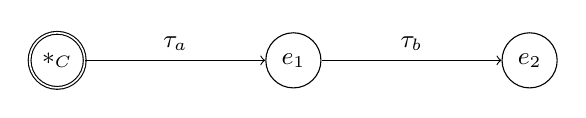
\begin{tikzpicture}[
  every node/.style={font=\small},
  v/.style={circle,draw,inner sep=1.5pt,minimum size=7mm},
  r/.style={circle,draw,double,inner sep=1.5pt,minimum size=7mm}
]
  \node[r] (root) at (0,0) {$*_C$};
  \node[v] (e1) at (3.0,0) {$e_1$};
  \node[v] (e2) at (6.0,0) {$e_2$};
  \draw[->] (root) -- node[above] {$\tau_a$} (e1);
  \draw[->] (e1) -- node[above] {$\tau_b$} (e2);
\end{tikzpicture}
\caption{The two possible incidence types for a deleted triangle in the one-bit,
height-two regime.  A triangle with one deleted edge is represented by an edge to the
formal component root; a triangle with two deleted edges is represented by an ordinary
edge between their vertices.  Deleting the root rows recovers the relative boundary
columns.}
\label{fig:incidence-types}
\end{figure}

The proposition turns the complete relative homology into elementary graph topology.
For a finite graph $G$, let $c(G)$ be its number of connected components and put
\[
  \beta_1(G)=|E(G)|-|V(G)|+c(G).
\]
Let $c_0(G_b(P))$ be the number of connected components containing no formal root.
Isolated roots are permitted and contribute neither a relative chain generator nor a
homology generator.

\begin{theorem}[complete integral relative homology]\label{thm:integral-homology}
For one-bit thinning of a finite poset of height at most two, the relative boundary
matrix $B$ is totally unimodular and
\begin{align}
  H_2(K,L;\Z)&\cong\Z^{\beta_1(G_b(P))},\label{eq:h2formula}\\
  H_1(K,L;\Z)&\cong\Z^{c_0(G_b(P))},\label{eq:h1formula}\\
  H_0(K,L;\Z)&=0.\label{eq:h0formula}
\end{align}
Consequently all integral relative homology groups are torsion-free, and for every
field $\Bbbk$,
\[
  \dim_{\Bbbk}H_2(K,L;\Bbbk)=\beta_1(G_b(P)),\qquad
  \dim_{\Bbbk}H_1(K,L;\Bbbk)=c_0(G_b(P)).
\]
\end{theorem}

\begin{proof}
An oriented graph-incidence matrix is totally unimodular.  One elementary proof is by
induction on a square submatrix: a column with at most one nonzero reduces the
determinant to a smaller minor, while if every column has two nonzeros then the
opposite signs make the row sum zero.  Deleting rows preserves total unimodularity.
Thus Proposition~\ref{prop:integral-incidence} gives the first claim.  This is the
ordinary graph-incidence phenomenon; more general relations between total
unimodularity and relative torsion are well established~\cite{DeyHiraniKrishnamoorthy2011}.

Consider one connected component of $G_b(P)$.  If it contains a root, deleting the
root row from its incidence matrix gives full row rank and zero cokernel; its kernel
is the integral cycle space.  If it contains no root, the matrix is the ordinary
incidence matrix of a connected graph, whose cokernel is $\Z$ and whose kernel is
again its cycle space.  Taking direct sums over graph components gives
\eqref{eq:h2formula}--\eqref{eq:h0formula}.  The universal coefficient theorem for
homology of the pair gives, for every field $\Bbbk$, a short exact sequence
\[
  0\longrightarrow H_k(K,L;\Z)\otimes_{\Z}\Bbbk
  \longrightarrow H_k(K,L;\Bbbk)
  \longrightarrow \operatorname{Tor}^{\Z}_1(H_{k-1}(K,L;\Z),\Bbbk)
  \longrightarrow0.
\]
The integral relative groups above are free, so the Tor term vanishes and the stated
field dimensions follow.
\end{proof}

\begin{remark}[novelty boundary]
The graph-incidence matrix, its total unimodularity, and the formulas for graph cycle
and component spaces are standard.  The candidate contribution is the recognition
that the particular Boolean thinning rule forces the relative simplicial boundary
into precisely this reduced-incidence form.  No new general matrix-tree theorem is
claimed.
\end{remark}

\section{The exact forest/collapse theorem}\label{sec:forest}

Call $G_b(P)$ a \emph{rooted forest} if it is acyclic and every connected component
contains exactly one formal root.  This includes isolated roots.

For later use, let $L\subseteq K$ be any same-vertex simplicial inclusion with
$\dim K\le2$.  Its \emph{relative support graph} $\Gamma(K,L)$ is the bipartite graph
whose left vertices are the deleted edges $E=K_1\setminus L_1$, whose right vertices
are the deleted triangles $T=K_2\setminus L_2$, and in which $e\in E$ is adjacent to
$\tau\in T$ exactly when $e\subset\tau$.  A perfect matching
$M=\{(e_i,\tau_i)\}$ is \emph{acyclic} if the directed graph on the matched pairs,
with an arrow $i\to j$ whenever $i\ne j$ and $e_i\subset\tau_j$, is acyclic.  This is
the usual acyclicity condition for the corresponding matching of the relative face
poset in this two-layer setting.

\begin{lemma}[two-layer matching--collapse lemma]\label{lem:matching-collapse}
Let $L\subseteq K$ be as above.  The following are equivalent:
\begin{enumerate}[label=(\roman*)]
\item $K$ collapses simplicially onto $L$ using only deleted edge--triangle pairs;
\item $\Gamma(K,L)$ has an acyclic perfect matching;
\item the poset of relative cells $K\setminus L$, ordered by inclusion, has a perfect
acyclic matching.
\end{enumerate}
\end{lemma}

\begin{proof}
A relative collapse sequence pairs every deleted triangle with the deleted edge removed
with it.  If the pair $(e_i,\tau_i)$ is removed at step $i$ and $e_i\subset\tau_j$
with $j\ne i$, then $\tau_j$ must already have been removed before step $i$; otherwise
$e_i$ would not be free.  Thus every arrow in the matched-pair digraph points strictly
backward in collapse order, so the resulting perfect matching is acyclic.

Conversely, let $M=\{(e_i,\tau_i)\}$ be an acyclic perfect matching.  Its
matched-pair digraph has a sink $i$.  By definition of sink, $e_i$ lies in no remaining
deleted triangle except $\tau_i$.  No retained triangle can contain a deleted edge,
because $L$ is a subcomplex, and there are no simplices above dimension two.  Hence
$e_i$ is a free face of $\tau_i$.  Collapse this pair and restrict $M$ to the remaining
relative cells.  The restricted matched-pair digraph is still acyclic, so iteration
removes all relative cells.  This proves (ii)$\Rightarrow$(i); condition (iii) is the
same matching condition expressed in the relative face poset.
\end{proof}

\begin{theorem}[one-bit height-two recognition theorem]\label{thm:main}
Let $P$ be a finite poset with $\posht(P)\le2$, let $b:P\to\{0,1\}$, define $Q$ by
\eqref{eq:binary-thinning}, and put $K=\D(P)$ and $L=\D(Q)$.  The following are
equivalent.
\begin{enumerate}[label=(\roman*)]
\item $H_*(K,L;\Ftwo)=0$.
\item $H_*(K,L;\Bbbk)=0$ for every field $\Bbbk$.
\item $H_*(K,L;\Z)=0$.
\item $G_b(P)$ is a rooted forest.
\item the poset of relative cells $K\setminus L$ admits a perfect acyclic matching
(equivalently, $\Gamma(K,L)$ has an acyclic perfect matching);
\item $K$ collapses simplicially onto $L$ by deleted edge--triangle pairs;
\item the inclusion $L\hookrightarrow K$ is a simple-homotopy equivalence;
\item the inclusion $L\hookrightarrow K$ is a homotopy equivalence.
\end{enumerate}
When these conditions hold and deleted cells are nonempty, $B$ is square and
$\det B=\pm1$ after compatible row and column orderings.
\end{theorem}

\begin{proof}
Theorem~\ref{thm:integral-homology} makes (i)--(iv) equivalent: vanishing is exactly
$\beta_1(G_b(P))=0$ and $c_0(G_b(P))=0$, which says that every graph component is a
tree containing its unique possible root.

Assume (iv).  Any nontrivial rooted tree has a nonroot leaf.  The corresponding
deleted edge $e$ lies in exactly one currently remaining deleted triangle $\tau$.
No retained triangle can contain a deleted edge, because $L$ is a subcomplex, and
there are no cells above dimension two.  Thus $e$ is a free face of $\tau$ in the
current complex.  Delete the pair $(e,\tau)$.  On $G_b(P)$ this is exactly pruning a
nonroot leaf and its incident graph edge, leaving a rooted forest.  Iteration removes
all deleted cells and proves (vi).  Recording the pairs in the pruning order yields an
acyclic perfect matching of the relative cells, proving (v) as well.

Lemma~\ref{lem:matching-collapse} gives the converse (v)$\Rightarrow$(vi) directly in
this two-layer situation; no general identification of arbitrary discrete-Morse
matchings with literal collapse sequences is being used.  A simplicial collapse gives
a simple-homotopy equivalence and
therefore a homotopy equivalence, so (vi)$\Rightarrow$(vii)$\Rightarrow$(viii).
Finally a homotopy equivalence induces an integral homology equivalence, giving
(viii)$\Rightarrow$(iii) and closing the cycle.

In the neutral nonempty case, \eqref{eq:relative-two-layer} has zero kernel and
cokernel, so $|E|=|T|$ and $B$ is an integral isomorphism.  Total unimodularity then
forces determinant $\pm1$.
\end{proof}

\begin{corollary}[greedy collapse algorithm]\label{cor:greedy}
After the deleted edges and triangles have been constructed, homotopy neutrality of a
one-bit height-two thinning can be decided in time linear in the size of the defect
incidence data: repeatedly remove a deleted edge incident to exactly one remaining
deleted triangle together with that triangle.  The procedure succeeds exactly when
all deleted cells are exhausted.
\end{corollary}

\begin{proof}
This is nonroot-leaf pruning in $G_b(P)$.  Equivalently, one may test directly that
each graph component is a tree with exactly one root.
\end{proof}

\begin{remark}
The theorem is stronger than a matrix-rank test for a particular coefficient field.
The extra force comes from the one-bit incidence structure, not from homology alone.
Section~\ref{sec:twobit} gives a unimodular relative boundary for which direct collapse
fails as soon as a second coordinate is allowed.
\end{remark}

\section{Structural sufficient conditions and logical examples}\label{sec:criteria}

The exact theorem above is specific to height two, but constructive sufficient
conditions are available in arbitrary height.  We record only the forms that will be
useful for interpreting Boolean observations.

\begin{proposition}[repair maps]\label{prop:repairmaps}
Let $P$ be any finite poset and $b:P\to\{0,1\}$.
\begin{enumerate}[label=(\alph*)]
\item If there is an order-preserving $\rho:P\to P$ such that
$\rho(p)\le p$ and $b(\rho(p))=0$ for every $p$, then
$\D(Q_b)\hookrightarrow\D(P)$ is a homotopy equivalence.
\item Dually, if there is an order-preserving $\lambda:P\to P$ such that
$p\le\lambda(p)$ and $b(\lambda(p))=1$ for every $p$, the same conclusion holds.
\end{enumerate}
\end{proposition}

\begin{proof}
In (a), $\rho$ is also monotone as a map $P\to Q_b$, and
$i\rho\le\operatorname{id}_P$ and $\rho i\le\operatorname{id}_{Q_b}$.  Pointwise
comparable monotone maps induce homotopic maps on order complexes, so $i$ and $\rho$
are homotopy inverses; see, for example, the comparable-map machinery in
Barmak~\cite{Barmak2011A}.  Part (b) is dual.
\end{proof}

Let $F=b^{-1}(0)$ and $T=b^{-1}(1)$.  Proposition~\ref{prop:repairmaps} immediately
gives the following closure-system criteria.

\begin{corollary}[floors, ceilings, and semilattice closure]\label{cor:closure}
Each of the following is sufficient for homotopy preservation.
\begin{enumerate}[label=(\alph*)]
\item For every $p\in P$, $F\cap\downarrow p$ has a greatest element.
\item For every $p\in P$, $T\cap\uparrow p$ has a least element.
\item $P$ is a finite join-semilattice, $F$ is join-closed, and
$F\cap\downarrow p\ne\varnothing$ for every $p$.
\item $P$ is a finite meet-semilattice, $T$ is meet-closed, and
$T\cap\uparrow p\ne\varnothing$ for every $p$.
\end{enumerate}
In (c) the repair is $\rho(p)=\bigvee(F\cap\downarrow p)$; in (d) it is
$\lambda(p)=\bigwedge(T\cap\uparrow p)$.
\end{corollary}

\begin{corollary}[Horn-type specialization]\label{cor:horn}
Suppose a realized-signature poset is a meet-subsemilattice of a Boolean cube and the
truth states of $b$ are the models of a Horn CNF in the old coordinates.  If every
realized signature lies below at least one such model, then the thinning preserves
homotopy type.  Dually, on a join-subsemilattice, a union-closed false region that is
lower cofinal gives a down-repair.
\end{corollary}

\begin{remark}
The closure properties of Horn and dual-Horn relations are classical~\cite{JeavonsCohenGyssens1997,Wild2017}.
The corollary is only their use as an explicit repair certificate; no blanket claim
that every Horn-defined observation is homotopy-neutral is intended.  The cofinality
and semilattice hypotheses are essential parts of the statement.
\end{remark}

\begin{example}[the Boolean diamond]\label{ex:diamond}
Let $P$ be the Boolean diamond on
$D=\varnothing$, $A=\{X\}$, $C=\{Y\}$, and $B=\{X,Y\}$.  Thus
$D<A<B$ and $D<C<B$.  The following four one-bit profiles illustrate the criteria and
the exact graph formula.
\begin{center}
\begin{tabular}{@{}ll>{\raggedright\arraybackslash}p{0.25\textwidth}>{\raggedright\arraybackslash}p{0.27\textwidth}@{}}
\toprule
observation & profile on $(D,A,C,B)$ & certificate & effect \\
\midrule
$X\vee Y$ & $0,1,1,1$ & isotone & $Q=P$ \\
$X\mathbin{\mathrm{XOR}}Y$ & $0,1,1,0$ & rooted tree & proper thinning; homotopy-neutral \\
$X\Leftrightarrow Y$ & $1,0,0,1$ & rooted tree / true ceiling & proper thinning; homotopy-neutral \\
$\neg(X\vee Y)$ & $1,0,0,0$ & one rootless component & topology changes \\
\bottomrule
\end{tabular}
\end{center}
For XOR the two deleted edges $A<B$ and $C<B$ are each anchored by a one-deletion
triangle, giving a rooted two-leaf tree.  XNOR is dual.  For NOR the root is isolated
and the three deleted-edge vertices form an unrooted path; Theorem~\ref{thm:integral-homology}
gives $H_1(K,L;\Z)\cong\Z$.
\end{example}

\section{A controlled chain corollary}\label{sec:chains}

The complete one-bit classification for a coarse chain is included only as a compact
order-theoretic corollary.  If $P=C_n$, two positions $i<j$ are incomparable in the
thinned order exactly when $b_i=1$ and $b_j=0$.  Hence the incomparability graph of
$Q$ is a bipartite Ferrers graph (the neighborhoods of the $1$-vertices are nested),
Writing $\operatorname{Inc}(Q)$ for this incomparability graph, pairwise comparable
sets in a poset are chains, so
\[
  \D(Q)=\operatorname{Ind}(\operatorname{Inc}(Q)),
\]
the independence complex of that Ferrers graph.  Dochtermann--Engstr\"om give the
corresponding contractible-versus-two-point homotopy dichotomy for independence
complexes of Ferrers graphs~\cite[Proposition~3.7]{DochtermannEngstrom2009}; related
Ferrers-graph topology is also developed by Claesson--Kitaev--Ragnarsson--Tenner
~\cite{ClaessonKitaevRagnarssonTenner2010}.  We therefore retain the result for its
explicit Boolean-word formulation and elementary beat-point proof, not as a novelty
claim.

\begin{theorem}[binary chain trichotomy]\label{thm:chain}
Let $P=C_n$ be the $n$-element chain and write $b_i=b(i)$.  Exactly one of the following
occurs.
\begin{enumerate}[label=(\alph*)]
\item The word $b_1\cdots b_n$ is nondecreasing.  Then $Q=P$.
\item The word is nonconstant and nonincreasing, hence $1^a0^{n-a}$ for some
$1\le a<n$.  Then $Q\cong C_a\sqcup C_{n-a}$; in particular the thinning changes
$H_0$.
\item In every other case, $Q$ is beat-contractible and
$\D(Q)\hookrightarrow\D(P)$ is a homotopy equivalence.
\end{enumerate}
Consequently there are $n+1$ profiles with $Q=P$, $n-1$ profiles for which the
thinning changes $H_0$, and $2^n-2n$ remaining profiles with $Q\ne P$ for which
$\D(Q)\hookrightarrow\D(P)$ is nevertheless a homotopy equivalence.
\end{theorem}

\begin{proof}
Case (a) is immediate from \eqref{eq:binary-thinning}.  In case (b), all comparisons
inside the initial $1$-block and final $0$-block survive, while every comparison from
the first block to the second is deleted, giving the stated disjoint union.

For case (c), if $b_1=0$ then the first chain element remains a global minimum of $Q$;
if $b_n=1$ the last remains a global maximum.  Either condition makes $\D(Q)$ a cone.
The only remaining endpoint pattern is $b_1=1$, $b_n=0$.  Since the word is not
nonincreasing, some $0$ occurs before a later $1$.  Remove the initial $1$-vertices one
at a time: for each such vertex, the first later $1$ is the least element of its strict
upper set in the current poset, so it is an up-beat point.  After these removals the
first remaining vertex has label $0$ and is a global minimum.  Thus $Q$ beat-reduces
to a point.  The coarse chain is also contractible, and any map between nonempty
contractible spaces is a homotopy equivalence.  Counting binary words gives the final
formula.
\end{proof}

\section{Sharpness I: two bits already fail}\label{sec:twobit}

For a general block thinning at height two, the relative complex still has the form
\eqref{eq:relative-two-layer}, but its columns need not be graph-incidence columns.
The relative support graph $\Gamma(K,L)$ introduced before
Lemma~\ref{lem:matching-collapse} is therefore the natural combinatorial object.
Perfect matchings are the \emph{fitting orientations} of higher-dimensional
rooted-forest theory in this special dimension~\cite{BernardiKlivans2016,DuvalKlivansMartin2016}.

\begin{proposition}[direct collapse and unique fitting orientation]\label{prop:unique-matching}
For any same-vertex block thinning $Q\subseteq P$ with $\posht(P)\le2$, the following are
equivalent:
\begin{enumerate}[label=(\roman*)]
\item $\D(P)$ collapses directly to $\D(Q)$ by deleted edge--triangle pairs;
\item the relative support graph has an acyclic perfect matching;
\item the relative support graph has exactly one perfect matching.
\end{enumerate}
The empty support graph has its unique empty matching and represents the identity
collapse.
\end{proposition}

\begin{proof}
Lemma~\ref{lem:matching-collapse} gives (i)$\Longleftrightarrow$(ii).  For a perfect
matching, a directed cycle in the matched-pair digraph is exactly an alternating cycle
of the bipartite support graph.  Flipping an alternating cycle gives a second perfect
matching.  Conversely, the symmetric difference of two distinct perfect matchings is
a nonempty disjoint union of alternating cycles.  Thus a perfect matching is acyclic
exactly when it is unique, proving (ii)$\Longleftrightarrow$(iii).  The
matching/fitting-orientation viewpoint is standard~\cite{Forman1998,BernardiKlivans2016}.
\end{proof}

We now give the sharp counterexample.  It is stated completely so that the existence
claim does not depend on the exhaustive search used later for minimality.

\begin{theorem}[seven-element two-bit counterexample]\label{thm:seven}
There is a seven-element poset $P$ of height two and a map
$\alpha:P\to\{0,1\}^2$ such that, for the coordinatewise thinned suborder $Q$,
\[
  \D(Q)\hookrightarrow\D(P)
\]
is an integral homology equivalence and a homotopy equivalence, but
$\D(P)\not\searrowrel\D(Q)$ by a relative elementary-collapse sequence.
\end{theorem}

\begin{proof}
Let $P$ be the transitive closure of the cover relations
\begin{equation}\label{eq:seven-covers}
\begin{split}
&0<2,\ 0<3,\ 0<4,\ 1<2,\ 1<4,\\
&2<5,\ 2<6,\ 3<5,\ 3<6,\ 4<5.
\end{split}
\end{equation}
Every maximal chain has three elements, so $\posht(P)=2$.  Define
\begin{center}
\begin{tabular}{c@{\qquad}ccccccc}
\toprule
$x$ & 0&1&2&3&4&5&6\\
\midrule
$\alpha(x)$ & 10&01&01&00&11&00&01\\
\bottomrule
\end{tabular}
\end{center}
The retained strict comparisons in $Q$ are
\begin{equation}\label{eq:seven-Q}
  (0,4),(1,2),(1,4),(1,6),(2,6),(3,5),(3,6).
\end{equation}
Order the deleted edges as
\[
\begin{array}{llll}
 e_1=(0,2),&e_2=(0,3),&e_3=(0,5),&e_4=(0,6),\\
 e_5=(1,5),&e_6=(2,5),&e_7=(4,5),
\end{array}
\]
and the deleted triangles as
\[
\begin{array}{llll}
 t_1=(0,2,5),&t_2=(0,2,6),&t_3=(0,3,5),&t_4=(0,3,6),\\
 t_5=(0,4,5),&t_6=(1,2,5),&t_7=(1,4,5).
\end{array}
\]
With the order orientation, the relative integral boundary is
\begin{equation}\label{eq:seven-matrix}
B=
\begin{bmatrix}
 1& 1& 0& 0& 0& 0& 0\\
 0& 0& 1& 1& 0& 0& 0\\
-1& 0&-1& 0&-1& 0& 0\\
 0&-1& 0&-1& 0& 0& 0\\
 0& 0& 0& 0& 0&-1&-1\\
 1& 0& 0& 0& 0& 1& 0\\
 0& 0& 0& 0& 1& 0& 1
\end{bmatrix},
\qquad \det B=-1.
\end{equation}
Thus $B$ is an integral isomorphism and the relative integral homology vanishes in
all degrees.  Hence the inclusion is an integral homology equivalence (and is a
homology equivalence over every field).

\begin{figure}[t]
\centering
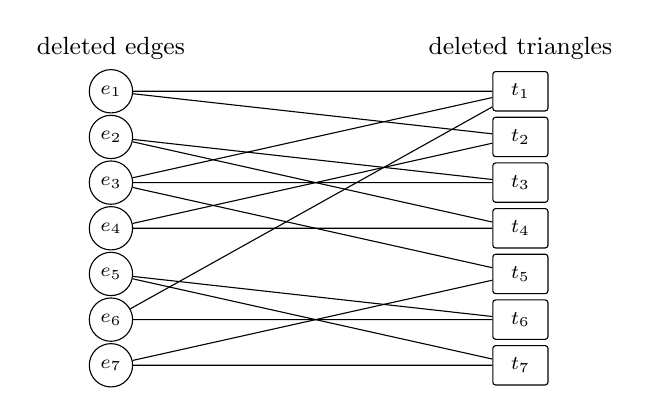
\begin{tikzpicture}[
  every node/.style={font=\scriptsize},
  leftv/.style={circle,draw,minimum size=5.5mm,inner sep=0.8pt},
  rightv/.style={rectangle,draw,rounded corners=1pt,minimum width=7mm,minimum height=5mm,inner sep=0.8pt}
]
  \foreach \i in {1,...,7} {
    \node[leftv] (e\i) at (0,{-(\i-1)*0.58}) {$e_{\i}$};
    \node[rightv] (t\i) at (5.2,{-(\i-1)*0.58}) {$t_{\i}$};
  }
  \draw (e1)--(t1) (e3)--(t1) (e6)--(t1);
  \draw (e1)--(t2) (e4)--(t2);
  \draw (e2)--(t3) (e3)--(t3);
  \draw (e2)--(t4) (e4)--(t4);
  \draw (e3)--(t5) (e7)--(t5);
  \draw (e5)--(t6) (e6)--(t6);
  \draw (e5)--(t7) (e7)--(t7);
  \node[font=\small] at (0,0.55) {deleted edges};
  \node[font=\small] at (5.2,0.55) {deleted triangles};
\end{tikzpicture}
\caption{Relative support graph of the seven-state two-bit example.  Every deleted
edge has degree at least two, so no relative elementary collapse can start.  The graph
nevertheless has three perfect matchings, listed in the text, whose signed determinant
contributions sum to $-1$.}
\label{fig:seven-support}
\end{figure}

The support graph has exactly three perfect matchings.  As permutations assigning to
row $e_i$ the column $t_{p(i)}$, they are
\[
\begin{split}
 &(1,4,3,2,7,6,5),\\
 &(2,3,1,4,7,6,5),\\
 &(2,3,5,4,6,1,7),
\end{split}
\]
where the displayed indices are one-based.  Their determinant contributions are,
respectively, $-1,+1,-1$, summing to $-1$.  This is precisely the kind of cancellation
among fitting orientations already present in the general higher-dimensional
rooted-forest framework~\cite{BernardiKlivans2016}; the point here is that two Boolean
coordinates can realize it inside this order-thinning problem.

More directly, the seven deleted-edge degrees into deleted triangles are
\[
  (2,2,3,2,2,2,2).
\]
No deleted edge is initially free.  Since every vertex is retained and there are no
simplices above dimension two, a relative elementary collapse would have to start by
pairing a deleted edge with its unique incident deleted triangle.  No such first move
exists.  Therefore $K\not\searrowrel L$.  Proposition~\ref{prop:unique-matching} gives
the same conclusion from the existence of three perfect matchings.

It remains to check homotopy equivalence.  Both endpoint posets beat-reduce to a point.
One valid reduction for $P$ is
\[
  3\downarrow0,\quad 4\uparrow5,\quad 0\uparrow2,\quad
  1\uparrow2,\quad 5\downarrow2,\quad 2\uparrow6,
\]
and for $Q$ it is
\[
  0\uparrow4,\quad 2\downarrow1,\quad 4\downarrow1,\quad
  1\uparrow6,\quad 5\downarrow3,\quad 3\uparrow6.
\]
Here $x\downarrow y$ means that $x$ is removed as a down-beat point with the indicated
extremal lower neighbor, and similarly for $\uparrow$.  Thus both order complexes are
nonempty and contractible.  Their inclusion is therefore a homotopy equivalence.
\end{proof}

The preceding theorem is a finite explicit proof.  Vertex minimality is a separate,
computer-assisted statement.

\begin{proposition}[computer-assisted vertex minimality]\label{prop:minimality}
No height-two two-bit counterexample of the type in Theorem~\ref{thm:seven} exists on
at most six vertices.  Consequently the seven-element example is vertex-minimal,
conditional only on the correctness of the exhaustive checker and its stated
enumeration model.
\end{proposition}

\begin{proof}[Exhaustive certificate]
For each $n\le6$, the checker enumerates every naturally labelled transitive relation
on $\{0,\ldots,n-1\}$ of height at most two and every one of the $4^n$ maps to
$\{0,1\}^2$.  Every finite poset admits a linear extension, so natural labellings cover
all isomorphism types, with harmless duplication.  For each pair it constructs the
coordinatewise thinned order, the deleted edges and triangles, and the relative
matrix over $\Ftwo$.  Relative acyclicity requires a square full-rank matrix.  For each
such neutral case, the program counts perfect matchings of the support graph and uses
Proposition~\ref{prop:unique-matching}: a neutral example fails direct collapse exactly
when the perfect matching is not unique.

The complete rerun produced
\begin{center}
\small
\begin{tabular}{@{}rrrrrr@{}}
\toprule
$n$ & posets & two-bit profiles & square cases & $\Ftwo$-neutral & max. matrix dim. \\
\midrule
1&1&4&4&4&0\\
2&2&32&25&25&0\\
3&7&448&256&256&1\\
4&39&9,984&4,174&4,174&2\\
5&330&337,920&104,114&103,562&4\\
6&4,117&16,863,232&3,865,228&3,767,044&8\\
\bottomrule
\end{tabular}
\end{center}
No neutral case through $n=6$ had more than one perfect matching.  The source, exact
outputs, and rerun logs are included with this paper; Section~\ref{sec:repro} records
the distinction between this exhaustive evidence and the analytic proof of
Theorem~\ref{thm:seven}.
\end{proof}

\begin{theorem}[sharp two-bit failure with certified minimality]\label{thm:twobit-sharp}
There exists a seven-element poset $P$ of height two and a map
$\alpha:P\to\{0,1\}^2$ such that, for the coordinatewise thinned suborder $Q$,
the inclusion $\D(Q)\hookrightarrow\D(P)$ is an integral homology equivalence and a
homotopy equivalence but $\D(P)\not\searrowrel\D(Q)$ by a relative elementary-collapse
sequence.  No such two-bit example exists on at most six vertices.

The existence assertion is the explicit mathematical construction of
Theorem~\ref{thm:seven}.  The vertex-minimality sentence is computer-assisted and is
exactly Proposition~\ref{prop:minimality}; it is not being presented as a separate
noncomputational proof.
\end{theorem}

\begin{corollary}[bit-count sharpness]\label{cor:bitsharp}
At height two, one bit is the maximal universal regime in which homology neutrality
forces direct collapse.  For every block size $r\ge2$, there are height-two
$r$-coordinate thinnings that are homology-neutral but do not collapse directly.
\end{corollary}

\begin{proof}
The one-bit assertion is Theorem~\ref{thm:main}, and the two-bit failure is
Theorem~\ref{thm:seven}.  For any $r>2$, append $r-2$ constant coordinates to the
seven-state two-bit labeling.  Coordinatewise comparability is unchanged, so the
thinned suborder and the same noncollapse certificate persist.
\end{proof}

\section{Sharpness II: greater height destroys one-bit rigidity}\label{sec:height}

The height hypothesis is independently sharp.  The following construction is elementary
but strong enough to show why no unrestricted one-bit analogue of
Theorem~\ref{thm:main} can hold.

\begin{theorem}[cone--whisker realization]\label{thm:cone-whisker}
Let $R$ be any nonempty finite poset and choose a minimal element $z\in R$.  Adjoin a
new greatest element $t$ to form $P=R\cup\{t\}$.  Define
\[
  b(z)=b(t)=0,\qquad b(x)=1\quad(x\in R\setminus\{z\}).
\]
Then the one-bit thinning $Q$ retains all comparisons of $R$ and precisely one new
comparison involving $t$, namely $z<t$.  Therefore
\begin{equation}\label{eq:cone-whisker}
  \D(P)=\operatorname{cone}(\D R),
  \qquad
  \D(Q)=\D(R)\cup_{\{z\}}[z,t],
\end{equation}
and $\D(Q)$ collapses onto $\D(R)$.  In particular,
\begin{equation}\label{eq:cone-homotopy}
  \D(Q)\hookrightarrow\D(P)\text{ is a homotopy equivalence}
  \quad\Longleftrightarrow\quad
  \D(R)\text{ is contractible},
\end{equation}
and for $k\ge1$,
\begin{equation}\label{eq:cone-relative}
  H_k(\D P,\D Q;\Z)\cong\widetilde H_{k-1}(\D R;\Z).
\end{equation}
\end{theorem}

\begin{proof}
Every comparison internal to $R$ survives: it is either $0\to1$ (when it starts at
$z$) or $1\to1$, apart from identities.  For $x\in R\setminus\{z\}$, the new
comparison $x<t$ is $1\to0$ and is deleted, while $z<t$ is $0\to0$ and survives.
Since $t$ is greatest in $P$, $\D(P)$ is a cone.  In $\D(Q)$ the edge $[z,t]$ is a
whisker and $t$ is a free vertex, so deleting it leaves $\D(R)$.  Equation
\eqref{eq:cone-homotopy} follows because the coarse complex is contractible, and
\eqref{eq:cone-relative} follows from the long exact sequence of the pair together
with \eqref{eq:cone-whisker}.
\end{proof}

\begin{corollary}[arbitrary refined homotopy type]\label{cor:arbitrarytype}
Within a contractible coarse order complex, one Boolean coordinate of unrestricted
height can realize, up to a single collapsible whisker, the order-complex homotopy type
of any nonempty finite poset.
\end{corollary}

\begin{corollary}[torsion in height three]\label{cor:torsion}
There are one-bit height-three thinnings with relative integral torsion.  In
particular, taking a height-two finite-poset model of $\mathbb{RP}^2$ as $R$ in
Theorem~\ref{thm:cone-whisker} gives
\[
  H_2(\D P,\D Q;\Z)\cong\Z/2.
\]
A 13-point projective-plane finite model is standard prior art~\cite{CianciOttina2018},
so this yields a 14-state example.  More generally, choosing $R$ with torsion in
reduced homology transfers that torsion one degree upward to the relative pair.
\end{corollary}

\begin{remark}
Theorem~\ref{thm:cone-whisker} also shows that integral homology neutrality need not
imply homotopy neutrality beyond height two: choose an acyclic but noncontractible
finite complex and take its face poset for $R$.  This is exactly the separation that
the rooted incidence structure rules out in Theorem~\ref{thm:main}.
\end{remark}

\section{Positioning and the logical-observation interpretation}\label{sec:logical}

\subsection{What is standard and what is specific here}

The mathematical ingredients used in the proofs have substantial prior art.
Finite-poset/order-complex methods and finite-space realization are classical
\cite{McCord1966,Barmak2011A,BarmakBook}.  Elementary collapse and acyclic matchings
belong to standard simple-homotopy and discrete-Morse theory
\cite{Forman1998,Kozlov2008}.  Higher-dimensional rooted forests, fitting orientations,
determinant weights, and cancellation among several fitting orientations are established
in the work of Bernardi and Klivans and related higher-dimensional tree theory
\cite{BernardiKlivans2016,DuvalKlivansMartin2016}.  Total-unimodularity and torsion
questions for simplicial boundary matrices likewise have a broader established
setting~\cite{DeyHiraniKrishnamoorthy2011}.  The Horn closure statements in
Section~\ref{sec:criteria} rely on classical closure properties rather than a new
classification of Horn logic~\cite{JeavonsCohenGyssens1997,Wild2017}.

The narrower candidate contribution of this paper is the exact recognition theorem
for the particular Boolean order-thinning rule: one coordinate plus height at most two
forces the defect into an ordinary reduced graph-incidence matrix, making coefficient
independence, rooted forests, perfect acyclic matchings of the relative cells, and actual collapse
all equivalent.  The seven-element two-bit example and the cone--whisker construction
then identify clean limits of that recognition theorem.  We make no claim that the
underlying graph, matching, or rooted-forest theories are new.

\subsection{Propositional logical topology interpretation}

In an observation-generated finite logical topology, one may pass to the Kolmogorov
quotient and regard the specialization structure as a finite poset of realized
observation signatures.  The same-carrier thinning model applies literally when the
new Boolean observation \emph{factors through the current $T_0$ quotient}: equivalently,
it is constant on every current observational-equivalence class and therefore does
not split a quotient point into several newly distinguishable states.  Under this
hypothesis, the new observation retains a coarse comparison exactly when its truth
value is nondecreasing along that comparison.  A single new observation is then
precisely the thinning \eqref{eq:binary-thinning}, and a simultaneous block that
factors through the current quotient is \eqref{eq:block-thinning}.

If a new observation separates worlds that were identified in the current quotient,
the refined $T_0$ carrier itself gains points; that operation is not merely a
same-carrier order thinning and is outside the literal scope of the theorems proved
here.

This statement should not be confused with McCord's theorem.  McCord's canonical map
from the order-complex realization to a finite $T_0$ space is a weak homotopy
equivalence~\cite{McCord1966}; it is not an assertion that every such realization map
is an ordinary homotopy equivalence.  Our main theorems are statements about the
order complexes $\D(Q)\subseteq\D(P)$.  Beat-point reductions are used only where they
explicitly contract the relevant finite posets/order complexes, and relative homology
computations are never presented as homotopy tests without an additional theorem such
as Theorem~\ref{thm:main}.

For the logical program, the operational message is correspondingly narrow.  A single
Boolean observation on a height-two current signature poset admits an exact, integral,
combinatorial safety test and an explicit collapse certificate.  Simultaneous
observation blocks do not inherit that equivalence automatically, and higher-height
models require genuinely stronger hypotheses such as the repair maps of
Section~\ref{sec:criteria}.

\section{Reproducibility and proof status}\label{sec:repro}

The manuscript is accompanied by a \texttt{reproducibility/} directory.  The principal
files are:
\begin{itemize}
\item \texttt{verify\_two\_bit\_height\_two\_counterexample.py}, an exact checker for
Theorem~\ref{thm:seven};
\item \texttt{two\_bit\_height2\_exhaustive.cpp}, the exhaustive checker used for
Proposition~\ref{prop:minimality}, with supplied and rerun outputs through $n=6$;
\item retained one-bit verifiers for the height-two matrix criterion, repair-map
sufficient conditions, chain classification, and repair-forest equivalence;
\item a reproducibility README and SHA-256 manifest.
\end{itemize}

There are two logically different kinds of claims.  The one-bit incidence theorem,
Theorem~\ref{thm:main}, the explicit seven-element construction, and the cone--whisker
theorem have mathematical proofs in the text.  The statement that seven vertices are
minimal for the two-bit failure is computer-assisted: the program exhausts the finite
search space through six vertices, but the paper does not disguise that enumeration as
a noncomputational proof.  The exact seven-state verifier independently reconstructs
the orders, the relative matrix, its determinant and $\Ftwo$ rank, the matching count,
the deleted-edge degrees, and the two beat reductions.

The retained one-bit checks are supplementary regression tests rather than foundations
for the proof.  In the post-audit rerun, the repair-forest verifier checked all
height-at-most-two naturally labelled posets through six vertices (4,117 posets at
$n=6$, 263,488 one-bit cases there) and reported all assertions passed.  The independent
height/homology and chain scripts likewise passed their stated ranges.  These finite
checks help guard transcription and implementation errors but are not substituted for
the proofs in Sections~\ref{sec:incidence}--\ref{sec:forest}.

\section{Conclusion}\label{sec:conclusion}

A one-bit observation on a height-two finite poset has an exactly classifiable
incidence defect.  The relative integral boundary is a reduced graph-incidence matrix,
so relative homology is torsion-free and determined by graph cycles and rootless
components.  In this regime, homology neutrality is not merely necessary for topological
neutrality: it forces a rooted forest and therefore an explicit simplicial collapse.

Both hypotheses are sharp.  Keeping height two but allowing two Boolean coordinates
already permits determinant cancellation among several fitting orientations; the
seven-element example is homology- and homotopy-neutral but admits no direct relative
collapse, and exhaustive computation certifies that six vertices do not suffice.
Keeping one bit but dropping the height bound allows arbitrary finite-poset homotopy
types inside a contractible coarse cone and relative torsion in height three.  These
two failures isolate the precise scope in which the one-bit forest theorem should be
used.

\begin{thebibliography}{99}

\bibitem{Barmak2011A}
J.~A. Barmak,
``On Quillen's Theorem A for posets,''
\emph{Journal of Combinatorial Theory, Series A} 118 (2011), 2445--2453.
\url{https://arxiv.org/abs/1005.0538}.

\bibitem{BarmakBook}
J.~A. Barmak,
\emph{Algebraic Topology of Finite Topological Spaces and Applications},
Lecture Notes in Mathematics 2032, Springer, 2011.

\bibitem{BarmakMinian2008}
J.~A. Barmak and E.~G. Minian,
``Simple homotopy types and finite spaces,''
\emph{Advances in Mathematics} 218 (2008), 87--104.

\bibitem{BernardiKlivans2016}
O. Bernardi and C.~J. Klivans,
``Directed rooted forests in higher dimension,''
\emph{Electronic Journal of Combinatorics} 23(4) (2016), P4.35.
DOI: 10.37236/5819.

\bibitem{CianciOttina2018}
N. Cianci and M. Ottina,
``Poset splitting and minimality of finite models,''
\emph{Journal of Combinatorial Theory, Series A} 157 (2018), 120--161.
DOI: 10.1016/j.jcta.2018.02.010.

\bibitem{ClaessonKitaevRagnarssonTenner2010}
A. Claesson, S. Kitaev, K. Ragnarsson, and B.~E. Tenner,
``Boolean complexes for Ferrers graphs,''
\emph{Australasian Journal of Combinatorics} 48 (2010), 159--173.

\bibitem{DochtermannEngstrom2009}
A. Dochtermann and A. Engstr\"om,
``Algebraic properties of edge ideals via combinatorial topology,''
\emph{Electronic Journal of Combinatorics} 16(2) (2009), R2.
DOI: 10.37236/68.

\bibitem{DeyHiraniKrishnamoorthy2011}
T.~K. Dey, A.~N. Hirani, and B. Krishnamoorthy,
``Optimal homologous cycles, total unimodularity, and linear programming,''
\emph{SIAM Journal on Computing} 40(4) (2011), 1026--1044.
\url{https://arxiv.org/abs/1001.0338}.

\bibitem{DuvalKlivansMartin2016}
A.~M. Duval, C.~J. Klivans, and J.~L. Martin,
``Simplicial and cellular trees,'' in \emph{Recent Trends in Combinatorics},
IMA Volumes in Mathematics and its Applications 159, Springer, 2016, 713--752.

\bibitem{Forman1998}
R. Forman,
``Morse theory for cell complexes,''
\emph{Advances in Mathematics} 134 (1998), 90--145.
DOI: 10.1006/aima.1997.1650.

\bibitem{Hatcher2002}
A. Hatcher,
\emph{Algebraic Topology}, Cambridge University Press, 2002.

\bibitem{JeavonsCohenGyssens1997}
P. Jeavons, D. Cohen, and M. Gyssens,
``Closure properties of constraints,''
\emph{Journal of the ACM} 44(4) (1997), 527--548.
DOI: 10.1145/263867.263489.

\bibitem{Kozlov2008}
D. Kozlov,
\emph{Combinatorial Algebraic Topology},
Algorithms and Computation in Mathematics 21, Springer, 2008.

\bibitem{McCord1966}
M.~C. McCord,
``Singular homology groups and homotopy groups of finite topological spaces,''
\emph{Duke Mathematical Journal} 33 (1966), 465--474.
DOI: 10.1215/S0012-7094-66-03352-7.

\bibitem{Wild2017}
M. Wild,
``The joy of implications, aka pure Horn formulas: Mainly a survey,''
\emph{Theoretical Computer Science} 658 (2017), 264--292.

\end{thebibliography}

\end{document}
